\section{Expansion, matter growth and cosmic structure}\label{sec:structure}
\subsection{Vacuum energy and expansion history}

\subsubsection{Vacuum density from the reference background}
For a spatially flat, late-time reference cosmology,
\begin{equation}
H^2(a)=H_0^2\bigl[\Om_ra^{-4}+\Om_ma^{-3}+\Om_\Lambda\bigr],\qquad
u_\Lambda^{\rm obs}=\frac{3H_0^2\Om_\Lambda c^2}{8\pi G}.
\end{equation}
Taking $H_0=67.4$ km s$^{-1}$ Mpc$^{-1}$, $\Om_m=0.315$, standard radiation, and flatness from the Planck base-$\Lambda$CDM reference \cite{Planck}, numerical evaluation gives
\begin{equation}\label{eq:lambdaobs}
\boxed{\begin{gathered}
\Om_\Lambda=0.684908,\qquad
u_\Lambda^{\rm obs}=5.2525\times10^{-10}\ \mathrm{J\,m^{-3}},\\
\Lambda_{\rm obs}=1.09076\times10^{-52}\ \mathrm{m^{-2}}\\
u_\Lambda^{\rm obs}=2.51894\times10^{-47}\ \Gev^4.
\end{gathered}}
\end{equation}
These values are \emph{derived from measured inputs}. An illustrative propagation of $\sigma(H_0)=0.5$ km s$^{-1}$ Mpc$^{-1}$ and $\sigma(\Om_m)=0.007$, holding the inputs independent and flatness fixed, gives a fractional uncertainty of $1.80\%$ for $u_\Lambda$. This observational-input estimate uses the stated diagonal covariance. A correlated posterior propagates through the same density relation with its full covariance matrix.

Equation~\eqref{eq:matching} defines the comparison with the QICT metric coefficients and independently fixed clock. The values in Eq.~\eqref{eq:lambdaobs} are observational reconstructions; the microscopic side of the comparison is the separately normalized response ratio in Eq.~\eqref{eq:operator-vacuum-invariant}.

\subsubsection{Dynamical dark energy}
If the physical metric sector contains a homogeneous dark-energy component with time-dependent equation of state $w(a)$, its density evolves as
\begin{equation}
\rho_{\rm de}(a)=\rho_{{\rm de},0}\exp\left[-3\int_1^a\frac{1+w(a')}{a'}\dd a'\right].
\end{equation}
The parameterization $w(a)=w_0+w_a(1-a)$ describes a two-parameter family of expansion histories. DESI DR2 tests this family jointly with other probes under specified likelihood assumptions \cite{DESI25}. Its coefficients, kinetic realization and perturbative sound speed are model inputs. The nonzero constant-volume QICT metric term selects the $w=-1$ member through Proposition~\ref{prop:w}.

\subsection{Growth of matter fluctuations and the power spectrum}

\subsubsection{Linear growth}\label{sec:linear-growth}
For smooth dark energy, negligible massive-neutrino scale dependence, subhorizon matter perturbations, and standard Poisson coupling, the growing mode satisfies
\begin{equation}\label{eq:growth}
\frac{\dd^2D}{\dd(\ln a)^2}+
\left(2+\frac{\dd\ln H}{\dd\ln a}\right)\frac{\dd D}{\dd\ln a}
-\frac32\Om_m(a)D=0.
\end{equation}
With the Planck-normalized reference background and the matter-era growing-mode initial condition at $a=0.01$, numerical integration, normalized to $D(z=0)=1$, gives
\begin{equation}
\boxed{D(z=0.5)=0.76894,\quad f(z=0.5)=0.76087,\quad f\sigma_8(z=0.5)=0.47449,}
\end{equation}
where $f=\dd\ln D/\dd\ln a$ and $\sigma_8(0)=0.811$ is the supplied normalization. This calculation adopts the GR scalar response. Section~\ref{sec:metric-scalar-joint} treats general quasistatic coupling and slip, and Section~\ref{sec:growth-inversion} derives their inversion from growth and lensing.

\begin{figure}[t]\centering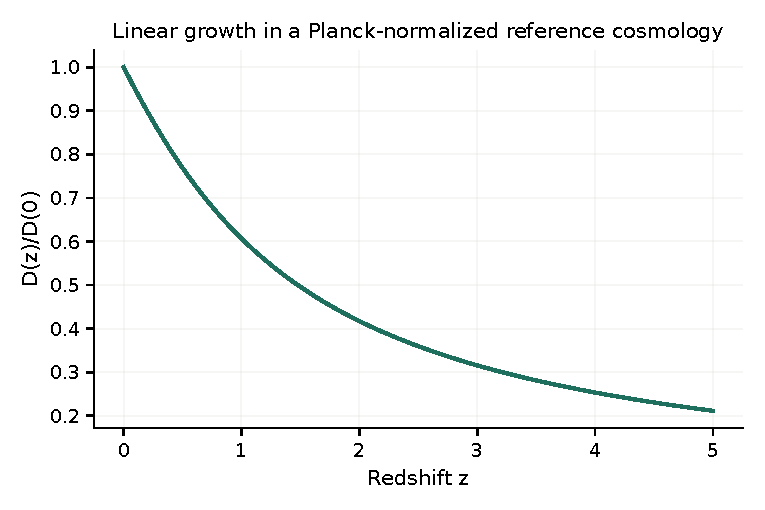
\includegraphics[width=.78\linewidth]{figures/growth_reference.pdf}\caption{Reference linear growth obtained from Eq.~\eqref{eq:growth}; the background and normalization are the stated Planck reference inputs.}\end{figure}

\subsubsection{A smooth matter-power reference spectrum}
The linear spectrum takes the form
\begin{equation}\label{eq:pk}
P_m(k,z)=A\,k^{n_s}T^2(k)D^2(z).
\end{equation}
For an inexpensive, explicitly approximate transfer calculation we use the baryon-corrected BBKS/Sugiyama smooth shape \cite{BBKS,Sugiyama}:
\begin{align}
T(q)&=\frac{\ln(1+2.34q)}{2.34q}
\bigl[1+3.89q+(16.1q)^2+(5.46q)^3+(6.71q)^4\bigr]^{-1/4},\\
q&=k/(h\Gamma_{\rm eff}),\quad
\Gamma_{\rm eff}=\Om_mh\exp\{-\Om_b[1+\sqrt{2h}/\Om_m]\},
\end{align}
Here $k$ is measured in $\Mp^{-1}$, as in the numerical implementation. The normalization is fixed by
\begin{equation}
\sigma_R^2=\frac{1}{2\pi^2}\int_0^\infty k^2P_m(k)W^2(kR)\dd k,\quad
W(x)=3\frac{\sin x-x\cos x}{x^3},
\quad \sigma_{8h^{-1}\Mp}=0.811.
\end{equation}
The numerical spectrum reproduces the supplied $\sigma_8$ under the stated physical-unit convention. BBKS describes a smooth linear transfer shape. Resolved acoustic features, nonlinear evolution and baryonic corrections belong to the corresponding Einstein--Boltzmann and matter-evolution model used in a survey likelihood.

\begin{figure}[t]\centering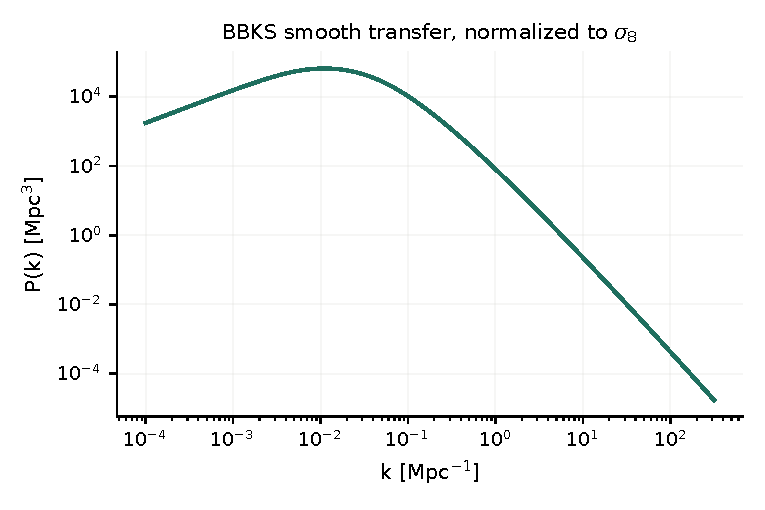
\includegraphics[width=.8\linewidth]{figures/matter_power_reference.pdf}\caption{Smooth BBKS-type reference spectrum normalized by the observed $\sigma_8$. The curve resolves the broad turnover in the smooth-transfer approximation.}\end{figure}

\subsection{Halo dynamics, mass functions, and galaxy populations}

\subsubsection{Halo abundance}\label{sec:halo-abundance}
For the Gaussian spherical-collapse reference with linear threshold $\delta_c=1.686$, the Press--Schechter estimate is
\begin{equation}
\frac{\dd n}{\dd\ln M}=\sqrt{\frac2\pi}\frac{\bar\rho_m}{M}
\frac{\delta_c}{\sigma(M)}\left|\frac{\dd\ln\sigma}{\dd\ln M}\right|
\exp\left[-\frac{\delta_c^2}{2\sigma^2(M)}\right].
\end{equation}
At $z=0$, the smooth reference spectrum gives $\dd n/\dd\ln M\simeq2.491\times10^{-3}$ Mpc$^{-3}$ at $M=10^{12}\msun$ and $2.704\times10^{-5}$ Mpc$^{-3}$ at $M=10^{14}\msun$. These are Press--Schechter estimates for the stated Gaussian-collapse and transfer assumptions \cite{PressSchechter,ShethTormen}. Survey counts also depend on the mass definition, selection function, cosmic variance, redshift-space mapping and halo occupation.

\begin{figure}[t]\centering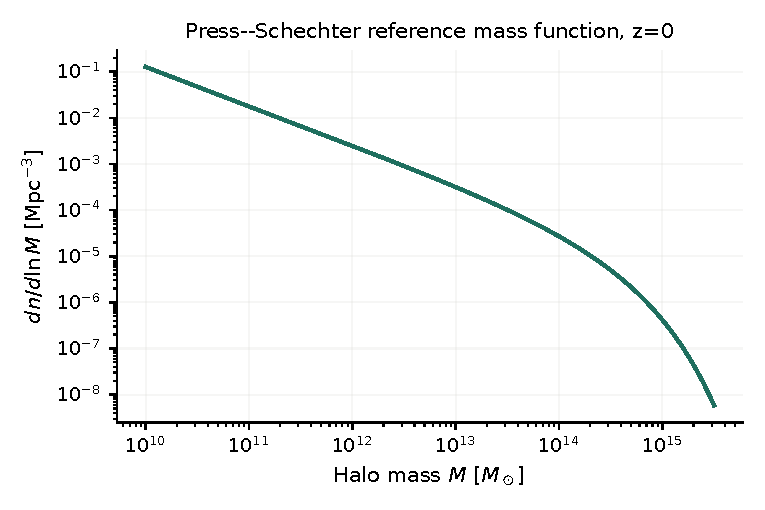
\includegraphics[width=.8\linewidth]{figures/halo_mass_function.pdf}\caption{Reference Press--Schechter halo abundance inferred from the smooth spectrum.}\end{figure}

\subsubsection{A radiation-consistent spherical-overdensity computation}\label{sec:spherical-collapse}
A uniform overdense region of fixed mass $M$ evolves in a smooth-$\Lambda$ background according to
\begin{equation}
\ddot R=-\frac{GM}{R^2}-\Omega_{r0}H_0^2a^{-4}R+\Omega_{\Lambda0}H_0^2R.
\end{equation}
Starting at $a_i=0.01$ with mass $M=10^{14}\msun$, $\delta_i=0.040$, radius fixed by mass conservation, and specified density-derivative initial velocity $\dot R_i=H_iR_i[1-\delta_i/(3(1+\delta_i))]$, the isolated top-hat reaches $R=0.01$ Mpc at $a=0.4614218$ in the reference background. The prescribed initial density derivative is $\delta_i^{\prime}=\delta_i$. The homogeneous radiation term is required by the same expansion background: setting $\delta_i=0$ recovers $R\propto a$. An independent density-contrast equation verifies the quoted threshold. The result describes one nonlinear, homogeneous overdensity with the stated initial data. Virial concentration, substructure and cosmological halo counts refer to distinct spatial observables.

\begin{figure}[t]\centering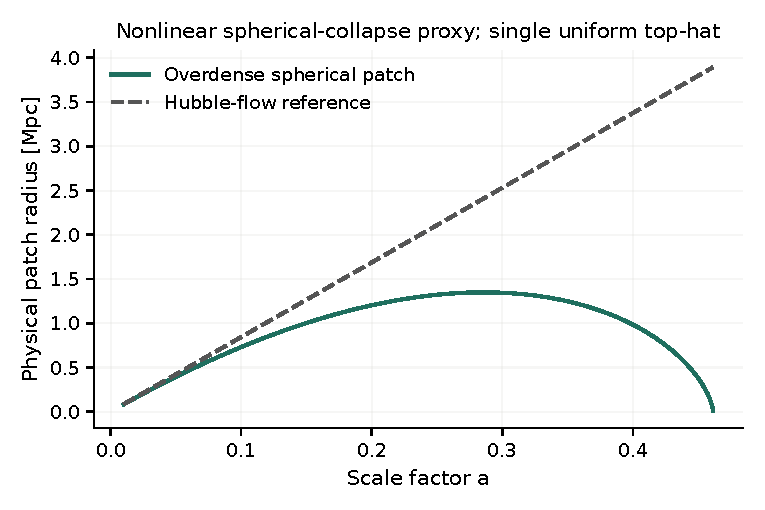
\includegraphics[width=.8\linewidth]{figures/spherical_collapse_reference.pdf}\caption{Numerical integration of an isolated spherical top-hat, compared with expansion at the background Hubble rate. The event is defined by the stated physical-radius threshold.}\end{figure}

\subsubsection{A transparent stellar-mass mapping}\label{sec:stellar-map}
The formation of observable galaxies requires star formation, feedback, metal enrichment, gas cooling, dust, and selection effects. For the limited purpose of illustrating the halo-to-stellar conversion, take
\begin{equation}
M_\star=\varepsilon_\star\frac{\Om_b}{\Om_m}M_h,
\quad \varepsilon_\star=0.05,\qquad
\phi_\star(M_\star)=\frac{\dd n}{\dd\log_{10}M_h}\left|\frac{\dd\log_{10}M_h}{\dd\log_{10}M_\star}\right|.
\end{equation}
For $M_h=10^{12}\msun$ the chosen constant-efficiency model gives $M_\star=7.816\times10^9\msun$. The chosen constant efficiency defines a deterministic halo-to-stellar mapping. Survey predictions extend it with scatter and a redshift-dependent star-formation model. Statistical galaxy clustering requires $P_g(k,z)=b_g^2(k,z)P_m(k,z)$ with a computed halo occupation or bias model and a likelihood against spectroscopic data. For example, the constant illustrative bias $b_g=1.5$ and the smooth linear spectrum yield
\begin{equation}
\xi_g(r)=\frac{b_g^2}{2\pi^2}\int_0^\infty k^2P_m(k,0)\frac{\sin kr}{kr}\dd k,
\quad \xi_g(10\,\Mp)=1.462405,\quad\xi_g(20\,\Mp)=0.466138.
\end{equation}
The oscillatory sine transform is evaluated adaptively over $0<k<\infty$, using a quadrature that resolves the oscillatory kernel. These values inherit the selected bias and observational normalization, and the smooth transfer sets their approximation domain separately from a resolved BAO calculation.

\begin{figure}[t]\centering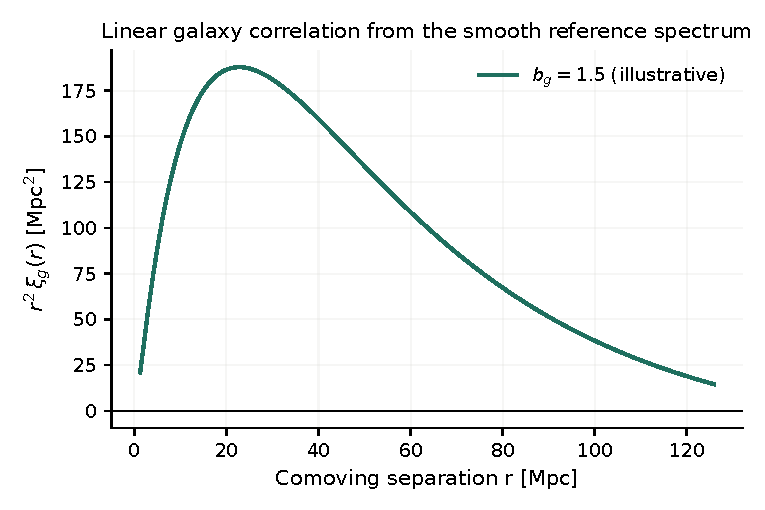
\includegraphics[width=.78\linewidth]{figures/galaxy_correlation_reference.pdf}\caption{Linear real-space galaxy correlation for a selected constant bias and BBKS smooth transfer. The observable is the real-space correlation before redshift-space and survey-window mapping.}\end{figure}

\begin{figure}[t]\centering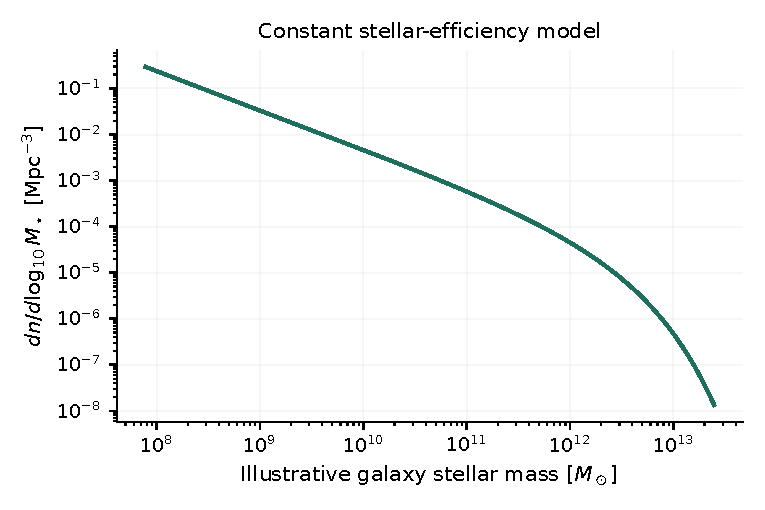
\includegraphics[width=.8\linewidth]{figures/stellar_mass_function.pdf}\caption{Stellar-mass function from a constant, explicitly chosen halo-to-stellar efficiency. The efficiency and background are independent inputs to this illustrative population model.}\end{figure}

\subsection{A three-dimensional gravitational clustering experiment}
\label{sec:pm3d}
The preceding halo calculation concerned a single spherical overdensity. To test gravitational clustering with spatially varying forces we additionally solved an explicit three-dimensional periodic particle--mesh (PM) system. The prescribed initial field defines a deterministic numerical experiment.

Let $\mathbf x$ be comoving coordinates in a periodic cube and $u=\ln a$. For pressureless particles in a flat matter-plus-$\Lambda$ background, the comoving evolution equations are
\begin{align}
\mathbf x'&=\mathbf v,\\
\mathbf v'&=-\left(2+\frac{H'}{H}\right)\mathbf v
-\frac32\Omega_m(a)\boldsymbol\nabla\nabla^{-2}\delta,
\qquad\delta=\frac{\rho-\bar\rho}{\bar\rho}.
\label{eq:pm}
\end{align}
We assigned and interpolated particle densities using cloud-in-cell weights, solved the periodic Poisson problem with a Fourier transform and advanced Eq.~\eqref{eq:pm} with a second-order midpoint integrator in $u$. The $k=0$ mode is set to zero, fixing the homogeneous potential gauge. The calculation uses $32^3$ equal-mass particles on a $32^3$ grid in a $100\,h^{-1}\,\mathrm{Mpc}$ box with 300 steps from $a=0.05$ to 1. The deliberately simple Zel'dovich initial displacement is a superposition of three coherent orthogonal plane waves with present-epoch linearly extrapolated amplitude 1.1. These three waves specify a coherent deterministic field.

The RMS grid-density contrast grows from $0.08547$ at $a=0.05$ to $3.1436$ at $a\approx0.5$ and $10.4690$ at $a=1$, with a final peak cell contrast of $1484.3$. The assignment conserves total particle mass to floating-point accuracy, and the deposited grid has mean $\langle\delta\rangle\simeq0$ at each stored epoch. These large cell contrasts follow from coherent nonlinear collapse and depend strongly on the selected particle and force resolution. Repeating the integration with 200 rather than 300 time steps changes the final grid RMS contrast by 0.25\% and the peak by 0.42\%; this comparison measures time discretization at fixed spatial resolution. The density statistics refer to this mesh and coherent initial field. Cosmological halo statistics additionally depend on the primordial ensemble, transfer function, box and force resolution, halo definition and baryonic dynamics.

\begin{figure}[t]
\centering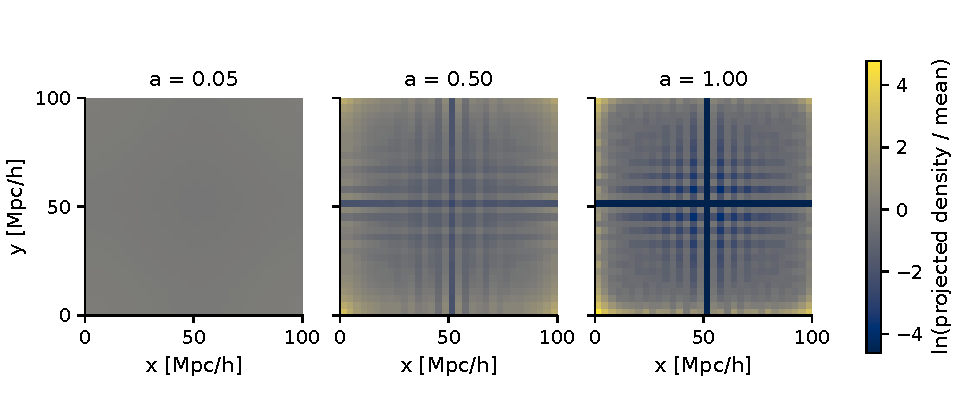
\includegraphics[width=\linewidth]{figures/particle_mesh_3d.pdf}
\caption{Evolution of the projected density in the numerical 3-D particle--mesh test at early, intermediate and late scale factors. The initial field contains coherent plane waves. All panels use the same logarithmic projected-density scale, with a display floor of 0.01 times the mean density.}
\end{figure}

\subsection{A solvable gas-regulator model for the stellar component}
\label{sec:gasreg}
A gas reservoir connects an imposed halo-accretion history to stellar growth. Suppose a halo accretes mass at a constant rate $\dot M_h$, a fraction $f_b$ reaches a gas reservoir, outflows remove $\eta_w\psi$, a fraction $\mathcal R$ of newly formed stellar mass is returned promptly, and the star formation law is $\psi=\epsilon_*M_g/t_d$. Then
\begin{equation}
\dot M_g=f_b\dot M_h-(1-\mathcal R+\eta_w)\frac{\epsilon_*}{t_d}M_g,
\qquad \dot M_*= (1-\mathcal R)\frac{\epsilon_*}{t_d}M_g.
\label{eq:gas-ode}
\end{equation}
For initially empty reservoirs, constant coefficients, $t_d>0$, $\epsilon_*>0$, $\eta_w\geq0$ and $0\leq\mathcal R<1$, let $\lambda=(1-\mathcal R+\eta_w)\epsilon_*/t_d>0$. The unique solution is
\begin{align}
M_g(t)&=\frac{f_b\dot M_h}{\lambda}\left(1-e^{-\lambda t}\right),\\
M_*(t)&=\frac{(1-\mathcal R)f_b\dot M_h}{1-\mathcal R+\eta_w}
\left[t-\frac{1-e^{-\lambda t}}{\lambda}\right],\\
\psi(t)&=\frac{f_b\dot M_h}{1-\mathcal R+\eta_w}\left(1-e^{-\lambda t}\right).
\label{eq:gas-sol}
\end{align}
The continuous limit $\epsilon_*\to0$ gives $M_g=f_b\dot M_h t$, $M_*=0$ and $\psi=0$. For the explicitly selected values $\dot M_h=50\,M_\odot\,\mathrm{yr}^{-1}$, $f_b=0.15633$, $\epsilon_*=0.05$, $t_d=0.1\,\mathrm{Gyr}$, $\mathcal R=0.4$, $\eta_w=1$ and $t=3\,\mathrm{Gyr}$, the solution gives $M_g=8.8841\times10^9M_\odot$, $M_*=5.4619\times10^9M_\odot$ and $\psi=4.4421\,M_\odot\,\mathrm{yr}^{-1}$. These are conditional predictions of the adopted gas-regulator model. The baryon fraction is computed from the previously adopted Planck reference parameters; the efficiencies and accretion history are chosen inputs. The calculation describes one well-mixed reservoir with instantaneous recycling and the stated constant coefficients. Resolved cooling, enrichment and radiative feedback define additional physical degrees of freedom in a spatial galaxy model.


\subsubsection{Time-dependent inflow and the baryon balance}
The gas-reservoir equation also has an exact solution for time-dependent coefficients. Let $I(t)=f_b(t)\dot M_h(t)$, $k_*(t)=\epsilon_*(t)/t_d(t)$ and $\lambda(t)=[1-\mathcal R(t)+\eta_w(t)]k_*(t)$, with $I,k_*,\eta_w\geq0$ and $0\leq\mathcal R<1$. For integrable coefficients, define $L(t)=\int_0^t\lambda(u)\dd u$. The integrating factor gives
\begin{equation}\label{eq:gas-green}
M_g(t)=M_g(0)e^{-L(t)}+\int_0^t I(s)e^{-[L(t)-L(s)]}\dd s.
\end{equation}
This is the unique solution and is nonnegative for nonnegative initial gas mass. The stellar and cumulative wind masses follow by integration of $(1-\mathcal R)k_*M_g$ and $\eta_wk_*M_g$, respectively. Adding the three equations proves the exact balance
\begin{equation}\label{eq:gas-balance}
M_g(t)+M_*(t)+M_w(t)
=M_g(0)+M_*(0)+M_w(0)+\int_0^t I(s)\dd s.
\end{equation}
For constant return and loading factors and initially empty reservoirs, $M_w=\eta_wM_* /(1-\mathcal R)$. The selected three-gigayear example therefore has $M_w=9.10314\times10^9M_\odot$ and cumulative gas inflow $2.34491\times10^{10}M_\odot$, consistent with the gas and stellar masses above. Equation~\eqref{eq:gas-green} shows explicitly how the consumption and outflow rates set the memory of the accretion history.
